\documentclass[11pt,twoside,a4paper]{report}
\usepackage{graphicx}



\begin{document}

\title{ID2216 Developing Mobile Applications\\Assignment 2 Report}
\author{Rafael Aldana (rafaelap@kth.se)\\Vincent Delitz (delitz@kth.se)\\Ruth Eriksson (ruthe@kth.se)}
\date{\today}
\maketitle

\newpage

%\begin{abstract}
%This is the abstract.
%\end{abstract}

\tableofcontents

%\listoffigures

%\listoftables

\newpage

\chapter{WebApp prototype}

After we have agreed to develop an application that helps users to find and offer SL cards in the previous assignment, we now focused on creating first prototypes and to get a preliminary structure for the application. Therefore, we created at the beginning a paper-based prototype and collected feedback from potential users and friends. Based on this, we then aimed to create a site-map of the different screens and views of our application and how the user travels through our app by creating a clickstream. Additionally, we then developed a new digital "paper-based" protoype of our app by using the online tool Balsamiq. \\In the following you can see, how we moved step by step forward and how our results of each step looked like.

\section{Paper prototype}

The very first step for creating the paper-based prototype was to think about which basic screens and functionalities does our user need. So, we took a paper and a pencil and started drawing the main views. Of course, we discussed a lot about, which features are really necessary for the first version of our app, since our goal is to build the app as slim and lean as possible. Furthermore, we tried to incorporate basic design principles of Android applications, so that the user will easily adapt to the usage of our application. Realized was this by using common design pattern of Android apps as well as a really clear structure. \\The outcome was that we have had a paper prototype based on eight different views, which had all a quite similiar design and an easy usability in our point of view. See the following pictures for more the detailed outcome.


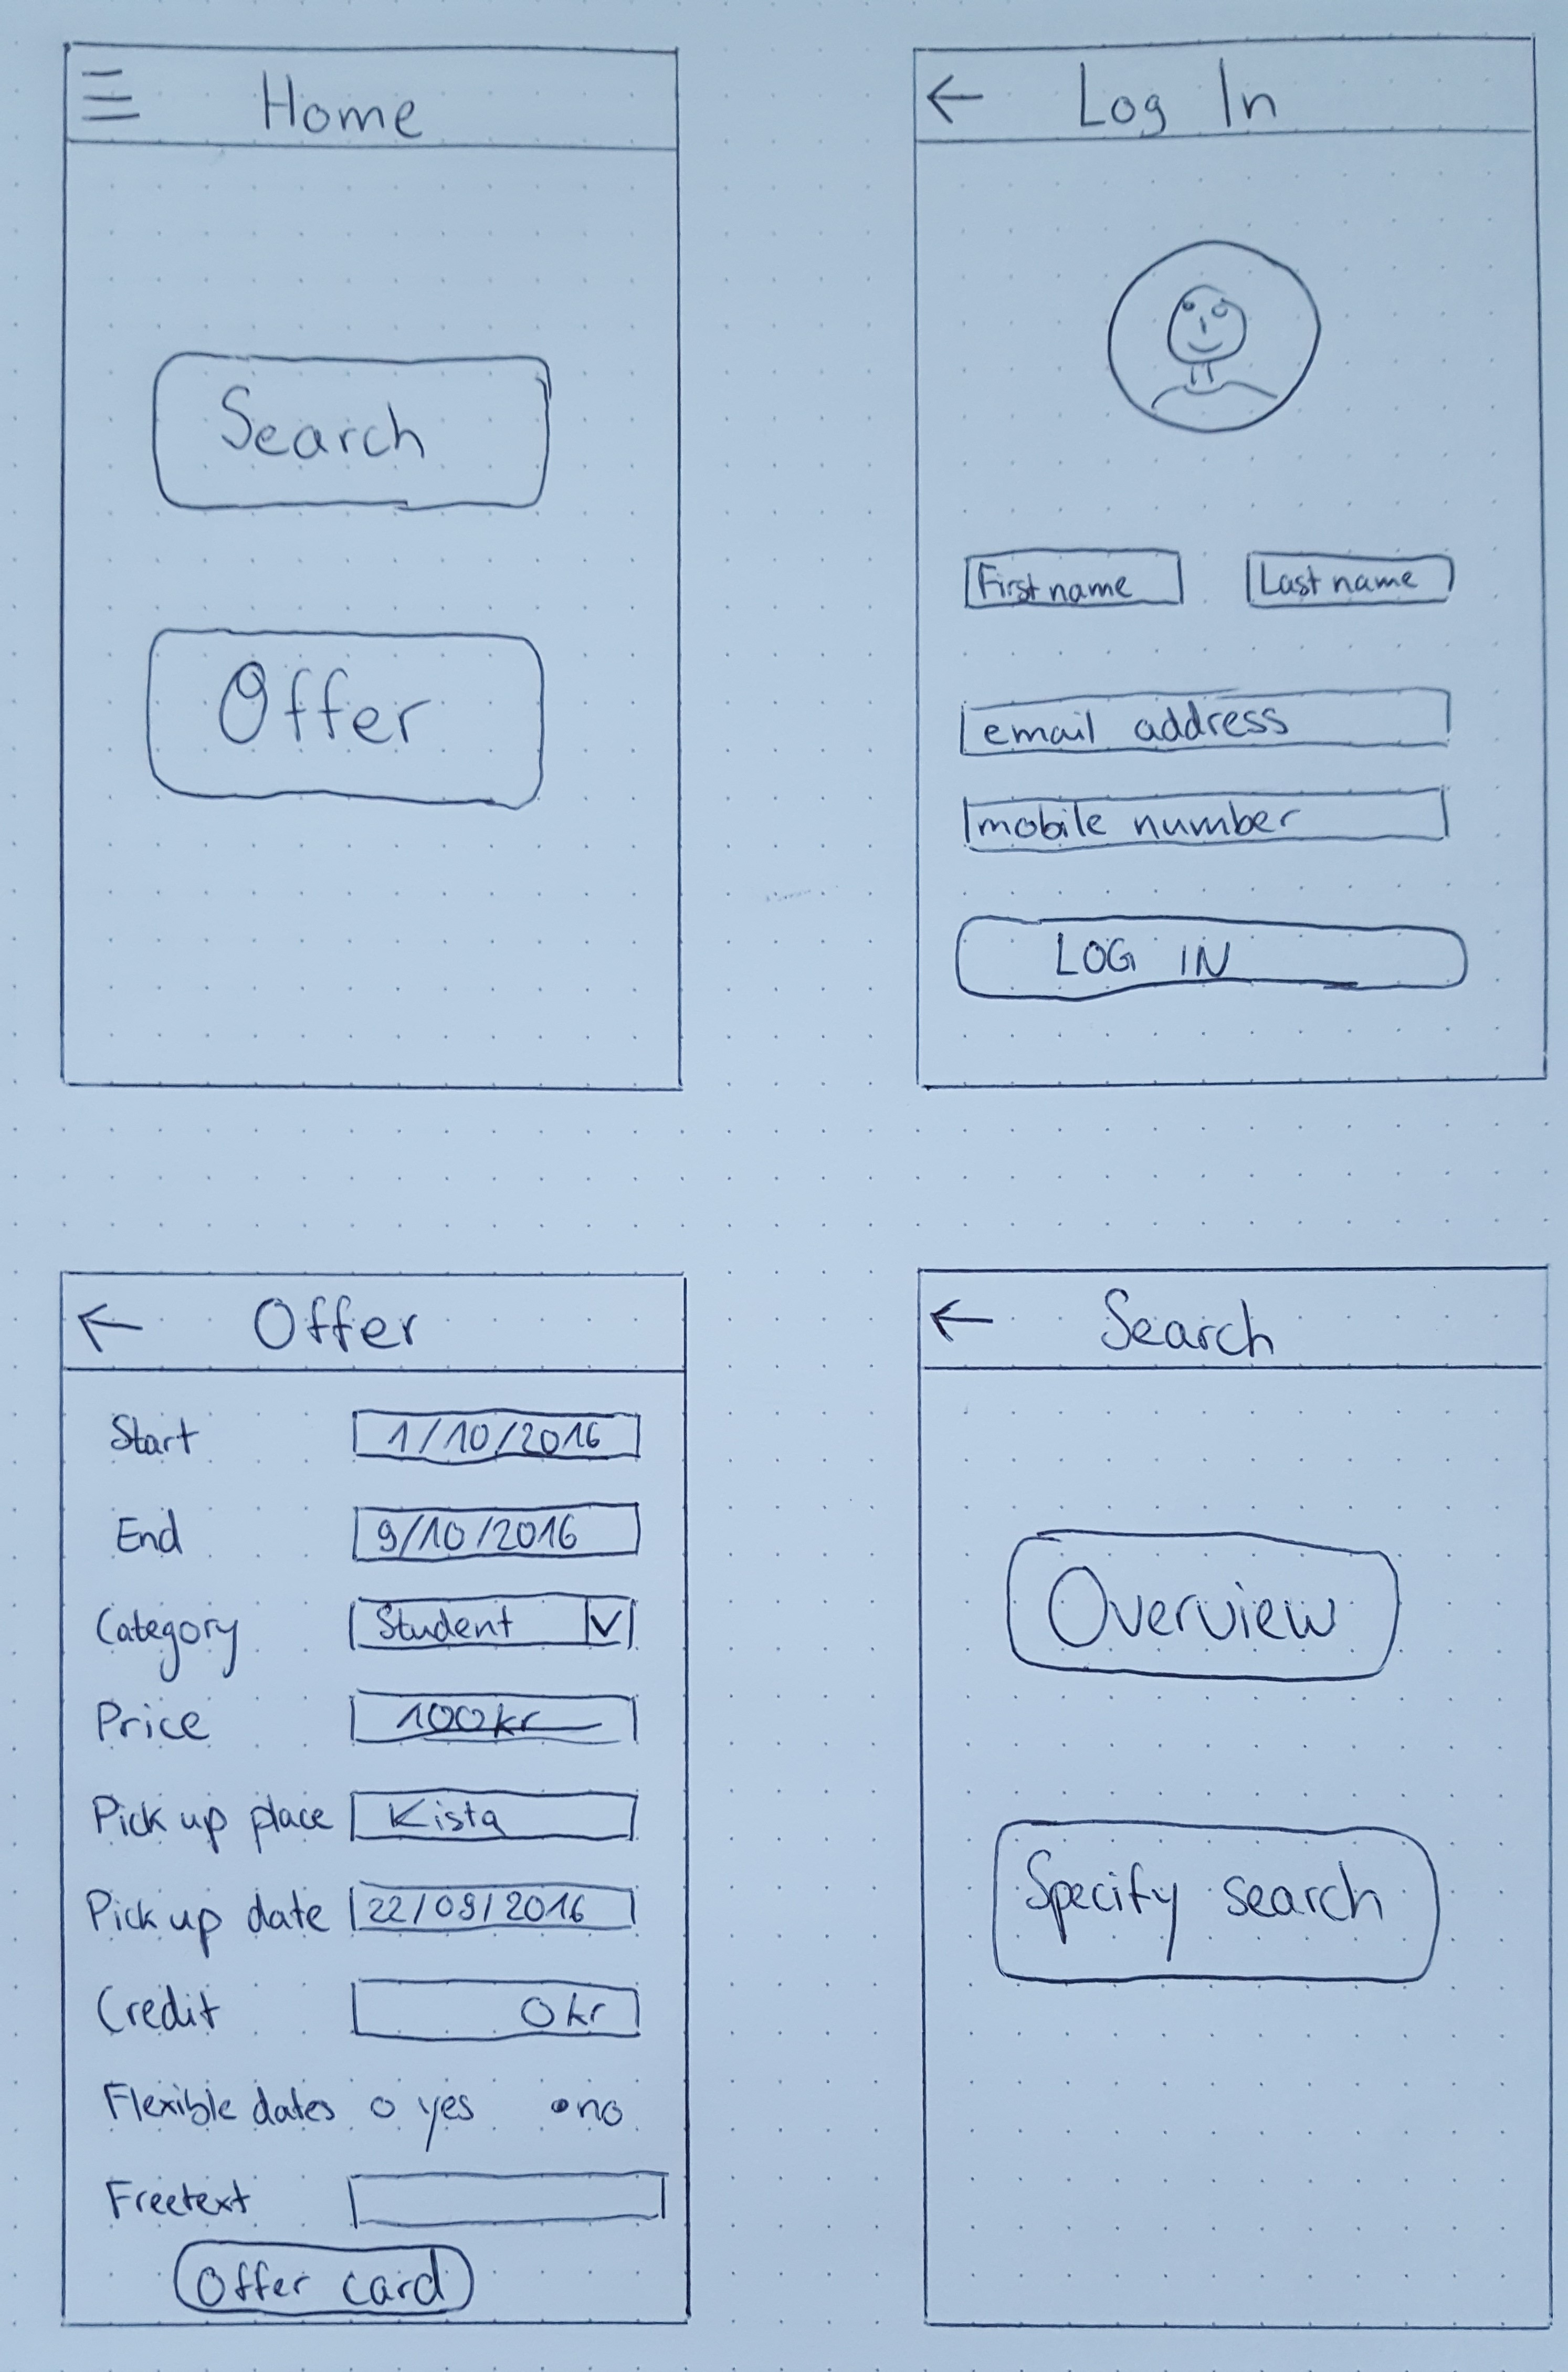
\includegraphics[scale=0.06]{Paper_prototype1.jpg}\\

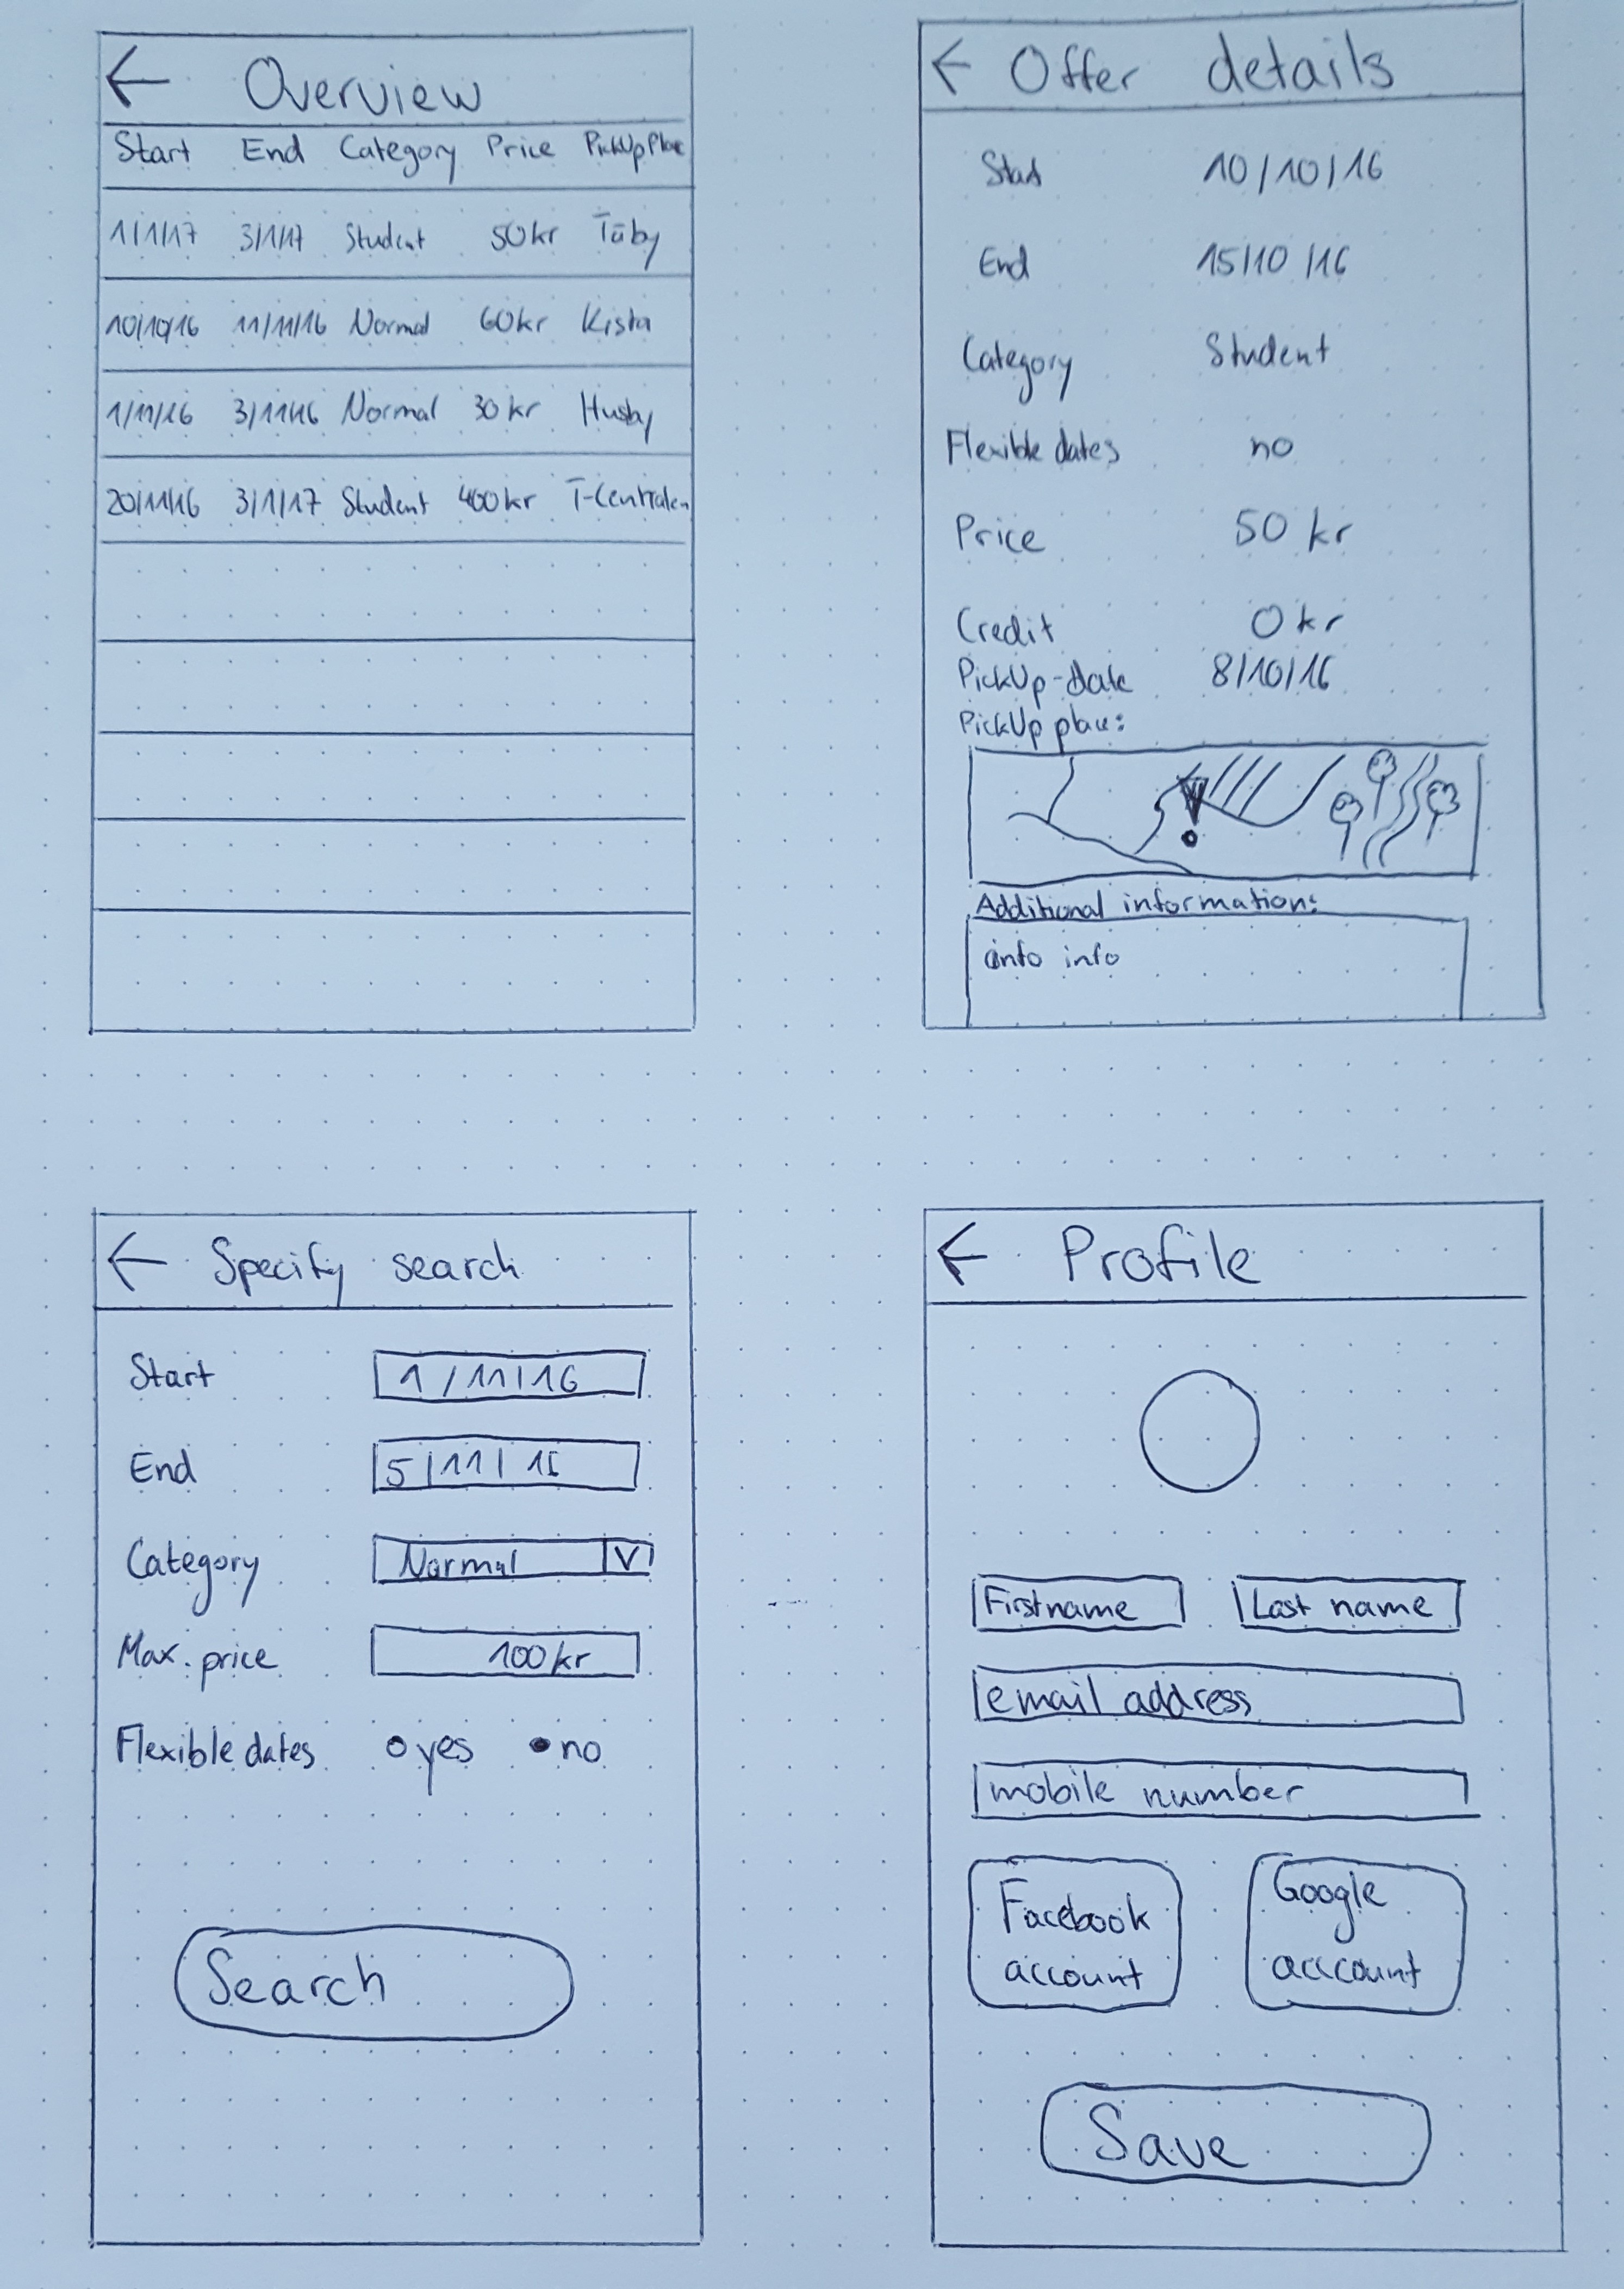
\includegraphics[scale=0.06]{Paper_prototype2.jpg}


\newpage
\section{Site-map}

After finalizing the paper-based prototype, we showed it to friends and other potential users in order to gather their impression and feedback. All in all, they liked the first prototype quite much, since it was also very simple and good in their opinion. Nevertheless, some also showed us that we missed little things or could improve the prototype at certain points. The following lists some major feedback points that we discovered:

\begin{itemize}

\item It would be nice to have start screen with the logo of our app, before reaching the home screen.

\item There should be a "Log out" button in the swipe menu on the left.

\item It would be cool to have settings screen, where you can define the date/time format and the displayed currency.

\item The offer details must definitely contain the user behind the offer and his contact details. Furthermore, it would be good to see how long he has been registered in the app.

\item A support tab in the swipe menu would also be nice, in case there are any questions or feedback for us.

\item As a matter of privacy, there should be an option if people searching for a SL card can see the mobile number of the seller or not. I think if someone sees the email address, this is fine, but the mobile number is quite sensitive.

\item It would be cool to have, maybe in a later stage, also a integrated chat system to contact the seller of a card.

\item It would nice to see a suggested price for the given validity period.

\item Be sure to implement the insertion of the date with the popup calendar.

\item Why so much data at login? Would it be enough with username and password to log in?

\item It would be nice to change Free Text for Extra Information or Comment or something more understandable.

\item Credit is not very clear and could be confuse with Price. What about Saldo?

\item It would be good to change Pick Up Place for Pick Up Station, if that is restricted to stations, we ensure that the buyer has a chance to check the validity of the card. In addition, it feels safer to meet that way.

\end{itemize}

\end{document}